\documentclass[10pt]{article}
\usepackage[margin=1in]{geometry}
\usepackage{amsfonts, amsmath, amssymb, amsthm} % AMS Math Packages
\usepackage{array, booktabs} % Extends the array and tabular environments
\usepackage{environ} % Interface for environments
\usepackage{setspace} % Paragraph indentation and line spacing
\usepackage{color} % Color control
\usepackage[x11names]{xcolor} % Color extensions 
\usepackage{soul} % Letter spacing, underlining, striking out 
\usepackage{fancybox, fancyhdr} % Variations of fbox and header/footer controls
\usepackage{tabularray} % Typeset tabulars and arrays with LaTeX3
\usepackage{graphicx} % Enhanced support for graphics 
\usepackage{enumitem} % Control layout of itemize, enumerate, description
\usepackage[position=top]{subcaption}
\usepackage{placeins}
\usepackage[colorlinks=true, linkcolor=blue, citecolor=blue]{hyperref}
% \hypersetup{pdfborder=0 0 0, citebordercolor=Gray0, urlbordercolor=Gray0, linkbordercolor=Gray0}
\usepackage[nameinlink]{cleveref}
\usepackage[at]{easylist}
\usepackage{enumitem}

% Picture notes
\newcommand{\Picnote}[1]{%
\vspace{-0.7em}
\flushleft
\hspace{6pt}
\hangindent=1.75em
\scriptsize
\emph{Notes:~}~#1
}

% Paragraph and itemize spacing
\setlength{\parskip}{0.75em}
\setlength{\parindent}{0pt}
\setlist[itemize]{topsep=0pt, itemsep=0pt}

\newcommand{\orange}[1]{\textcolor{orange}{#1}}
\allowdisplaybreaks

\title{Dogs of New York City}
\author{Cody Cook}
\date{\today}

\begin{document}
\maketitle  

% All figures/tables should be in the inputs folder, not another part of the repository 
There are 36143 dogs in the dataset. After filtering to only keep dogs with a name and breed, there are 31496 dogs. \Cref{fig:top_breeds_and_names} shows the top 10 most popular dog breeds and names in NYC. 

\begin{figure}[htpb]
    \caption{Popular names and breeds}
    \label{fig:top_breeds_and_names}
    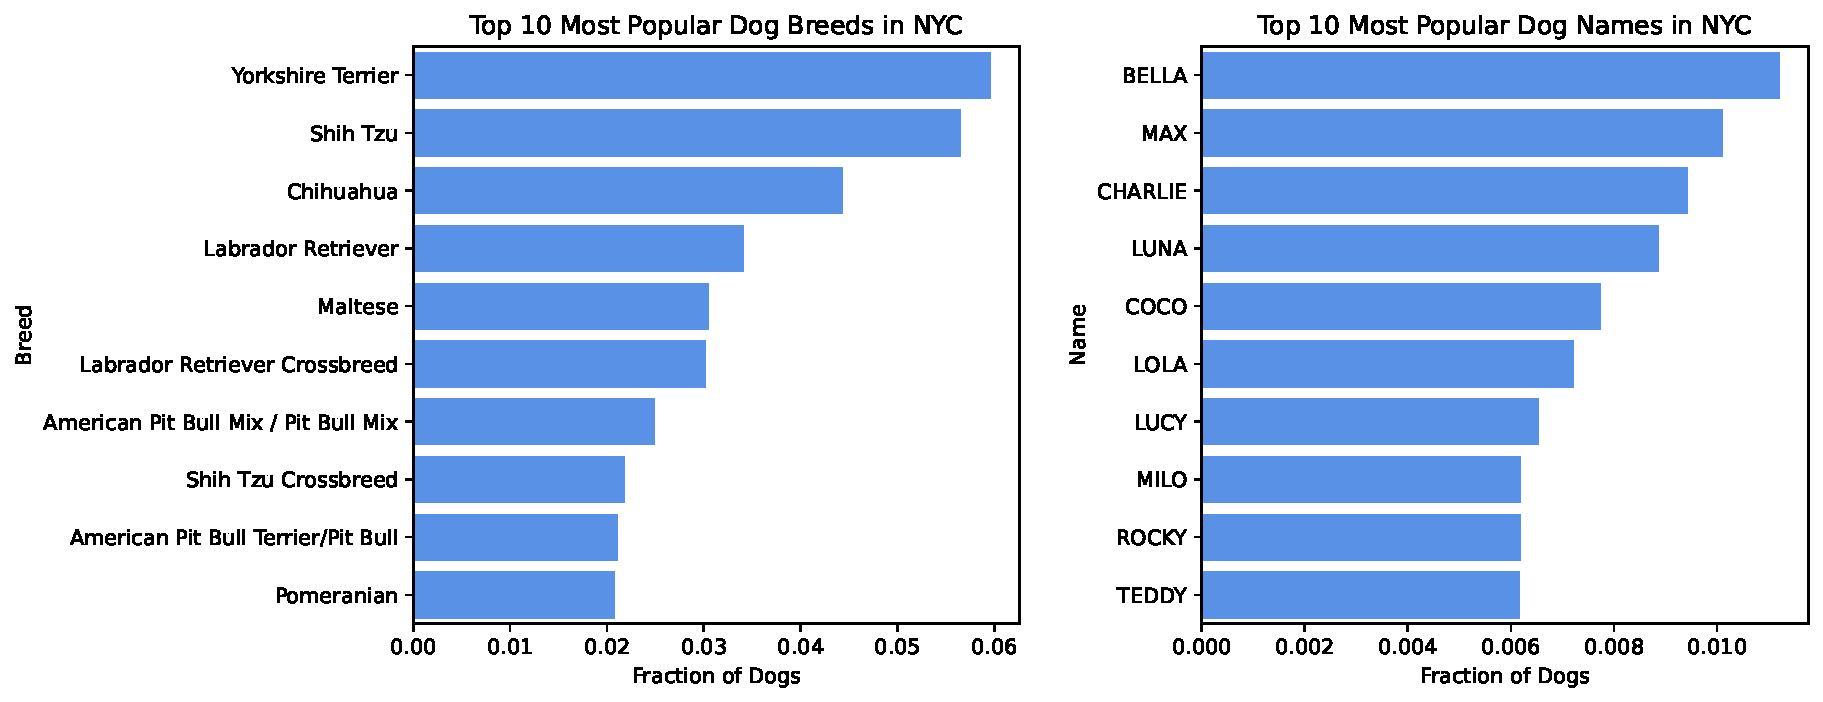
\includegraphics[width=1\textwidth]{input/top_breeds_and_names.pdf}
\end{figure}

\end{document}